% Original photograph with compact numbered markers; key stays in the caption.
\IfFileExists{figures/hazbot_prototype.pdf}{%
\begin{figure}[t]
\centering
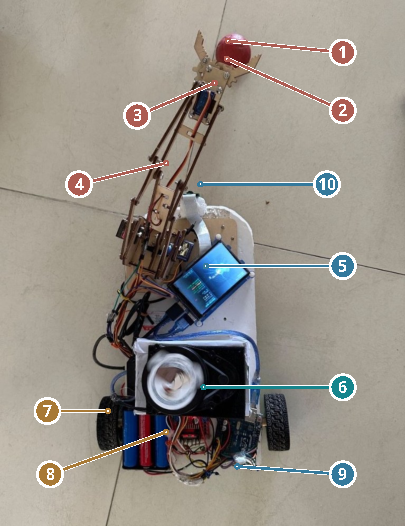
\includegraphics[width=0.78\columnwidth]{hazbot_prototype.pdf}
\caption{Physical HazBot prototype. Markers identify: 1, ball surrogate; 2, gripper; 3, servo; 4, arm linkage; 5, Raspberry Pi with GPIO-mounted display; 6, LiDAR; 7, drive wheel; 8, battery cells; 9, control electronics; 10, camera at the end of the white CSI ribbon.}
\label{fig:prototype}
\end{figure}
}{}

\IfFileExists{figures/hazbot_front.pdf}{%
\begin{figure}[t]
\centering
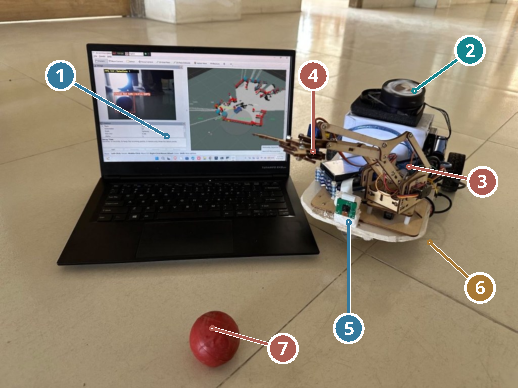
\includegraphics[width=\columnwidth]{hazbot_front.pdf}
\caption{Front view with laptop visualization. Markers identify: 1, laptop visualization; 2, LiDAR; 3, arm linkage; 4, gripper; 5, CSI camera; 6, mobile base; 7, ball surrogate.}
\label{fig:front}
\end{figure}
}{}
